\documentclass[11pt]{article}

\usepackage[margin=1in]{geometry}
\usepackage{graphicx}
\usepackage{amsmath,amssymb}
\usepackage{booktabs}
\usepackage{hyperref}
\usepackage{caption}
\usepackage{subcaption}
\usepackage{enumitem}
\usepackage{xcolor}
\usepackage{float}

\title{Certified and Empirical Uncertainty Quantification\\in Matmul-Free Language Models via Bound Propagation}
\author{%
    \texttt{steven202} \\
    DATA 691 -- Trustworthy AI -- Final Project
}
\date{May 2026}

\begin{document}
\maketitle

\begin{abstract}
Quantifying uncertainty in large language model (LLM) outputs is essential for trustworthy deployment. Formal verification methods such as Interval Bound Propagation (IBP) provide \emph{certified} guarantees that model predictions stay within provable bounds under input perturbations. We apply IBP and Monte Carlo empirical bounds to MMfreeLM (370M--2.7B parameters), a family of efficient recurrent language models, by adding $L_\infty$ perturbations to continuous token embeddings and propagating bounds through the network. We find that certified IBP bounds explode after a single layer due to compounding conservatism in normalization and recurrent operations, while Monte Carlo empirical sampling yields stable, interpretable uncertainty estimates. Larger models do not necessarily exhibit higher uncertainty: the 1.3B variant is 2--3$\times$ more sensitive to embedding perturbations than both the 370M and 2.7B models. Our results characterize the ``certification gap'' for recurrent LLMs and provide practical guidance for robustness analysis.
\end{abstract}

\section{Introduction}

Large language models are increasingly deployed in high-stakes applications, yet their robustness to small input variations remains poorly understood. A model that produces radically different outputs under imperceptible input changes is untrustworthy. Uncertainty quantification (UQ) --- measuring output variability under bounded perturbations --- is therefore central to trustworthy AI.

Two paradigms exist for UQ under perturbations: \textbf{empirical methods} (Monte Carlo sampling) estimate output variation by sampling perturbed inputs but provide no formal guarantees; \textbf{certified methods} (interval bound propagation, IBP) provide provable bounds over \emph{all} perturbations within a set, but may be loose.

We apply both paradigms to MMfreeLM~\cite{hgrn2024}, a family of efficient recurrent LMs that replace dense matrix multiplications with ternary weight quantization. We study three sizes (370M, 1.3B, 2.7B parameters) and ask: \emph{How much does the output distribution shift when token embeddings are perturbed within an $L_\infty$ ball of radius $\varepsilon$?}

Our contributions are: (1) the first application of formal bound propagation to matmul-free LLMs for UQ; (2) demonstration that certified IBP bounds explode due to normalization layers in recurrent architectures; (3) empirical UQ results showing a non-monotonic relationship between model size and sensitivity to perturbations; and (4) a reusable open-source implementation.

\section{Methods}

\subsection{Problem Formulation}

Let $f: \mathbb{R}^{L \times d} \to \mathbb{R}^{L \times V}$ be a language model mapping $L$ token embeddings (each in $\mathbb{R}^d$) to logits over vocabulary $V$. For nominal embedding $\mathbf{x}$, define the $L_\infty$ perturbation ball $\mathcal{B}_\varepsilon(\mathbf{x}) = \{\mathbf{x}' : \|\mathbf{x}' - \mathbf{x}\|_\infty \leq \varepsilon\}$. We seek bounds $f^L, f^U$ such that $f^L \leq f(\mathbf{x}') \leq f^U$ (element-wise) for all $\mathbf{x}' \in \mathcal{B}_\varepsilon(\mathbf{x})$. The bound width $f^U - f^L$ quantifies output uncertainty.

\subsection{Interval Bound Propagation (Certified)}

IBP~\cite{gowal2018} propagates interval tensors $[\mathbf{h}^L, \mathbf{h}^U]$ layer-by-layer. For an affine layer $\mathbf{h} \mapsto \mathbf{W}\mathbf{h} + \mathbf{b}$:
\begin{equation}
\mathbf{h}'^L = \mathbf{W}\boldsymbol{\mu} - |\mathbf{W}|\mathbf{r} + \mathbf{b}, \quad
\mathbf{h}'^U = \mathbf{W}\boldsymbol{\mu} + |\mathbf{W}|\mathbf{r} + \mathbf{b}
\end{equation}
with $\boldsymbol{\mu} = (\mathbf{h}^U + \mathbf{h}^L)/2$, $\mathbf{r} = (\mathbf{h}^U - \mathbf{h}^L)/2$.
For monotonic activations $\sigma$: $\mathbf{h}'^L = \sigma(\mathbf{h}^L)$, $\mathbf{h}'^U = \sigma(\mathbf{h}^U)$.

We implement IBP for the MMfreeLM architecture following the CROWN-IBP pattern~\cite{zhang2020}, handling:
\begin{itemize}[nosep]
    \item \textbf{BitLinear}: treated as standard linear for bound propagation (ternary quantization adds bounded $\pm 0.5$ error).
    \item \textbf{RMSNorm}: interval analysis of $x/\text{rms}(x)\cdot w$, bounding the RMS denominator independently per dimension.
    \item \textbf{Sigmoid, SwiGLU}: monotonic element-wise IBP and 4-corner interval arithmetic.
    \item \textbf{Gated recurrence} $o_t = f_t \odot o_{t-1} + i_t$ with $f_t \in (0,1)$: 4-corner enumeration at each time step over $(f_t, o_{t-1}, i_t)$.
\end{itemize}

\subsection{Monte Carlo Empirical Bounds (Practical)}

We sample $K=50$ points uniformly from $\mathcal{B}_\varepsilon(\mathbf{x})$ and take element-wise extrema:
\begin{equation}
f^L \approx \min_{k=1}^K f(\mathbf{x}^{(k)}), \quad f^U \approx \max_{k=1}^K f(\mathbf{x}^{(k)})
\end{equation}
These are \emph{not} certified but provide practical estimates. We also compute a two-pass baseline using only the corner points $\mathbf{x} \pm \varepsilon$.

\subsection{Metrics}

\textbf{Mean bound width}: $\frac{1}{LV}\sum_{i,j} |f^U_{ij} - f^L_{ij}|$. \\
\textbf{Top-1 stability}: fraction of positions where $\arg\max f^L = \arg\max f^U$. \\
\textbf{Certified margin}: $f^L_c - \max_{j \neq c} f^U_j$ for predicted class $c$.

\section{Experimental Setup}

\textbf{Models}: MMfreeLM-370M (24 layers, $d{=}1024$), MMfreeLM-1.3B (24 layers, $d{=}2048$), MMfreeLM-2.7B (32 layers, $d{=}2560$) from HuggingFace.\footnote{\texttt{ridger/MMfreeLM-370M}, \texttt{ridger/MMfreeLM-1.3B}, \texttt{ridger/MMfreeLM-2.7B}}

\textbf{Prompts}: Five prompts spanning factual knowledge, sentence completion, and open-ended generation (max 32 tokens).

\textbf{Perturbation}: $L_\infty$ noise on continuous token embeddings at $\varepsilon \in \{0.001, 0.005, 0.01, 0.05, 0.1\}$ ($\sim$0.1\%--10\% of typical embedding magnitude).

\textbf{Implementation}: Custom bound propagation layer built on PyTorch 2.2 and \texttt{mmfreelm}, run on a single NVIDIA GPU (float16 inference, float32 bound computation).

\section{Results}

\subsection{Certified IBP Bounds Explode}

Certified IBP bounds become numerically unstable within the first transformer block, producing NaN at layer 1 for all $\varepsilon > 0$ across all model sizes. The root cause is the conservative RMSNorm interval analysis: independently bounding the RMS denominator per dimension allows $x_i/\text{rms}(\mathbf{x})$ to reach values $\sim$1000$\times$ wider than physically realizable. The gated recurrence $o_t = f_t o_{t-1} + i_t$ compounds this over time steps, and the 24--32 layer depth amplifies the bound width exponentially.

This negative result demonstrates that \textbf{vanilla IBP is insufficient for certifying deep recurrent LLMs}, motivating tighter bound propagation techniques.

\subsection{Empirical Uncertainty Estimates}

Figure~\ref{fig:bound_width} shows mean bound width vs.\ $\varepsilon$ for all three model sizes. Table~\ref{tab:results} provides representative values at $\varepsilon{=}0.01$.

\begin{figure}[H]
    \centering
    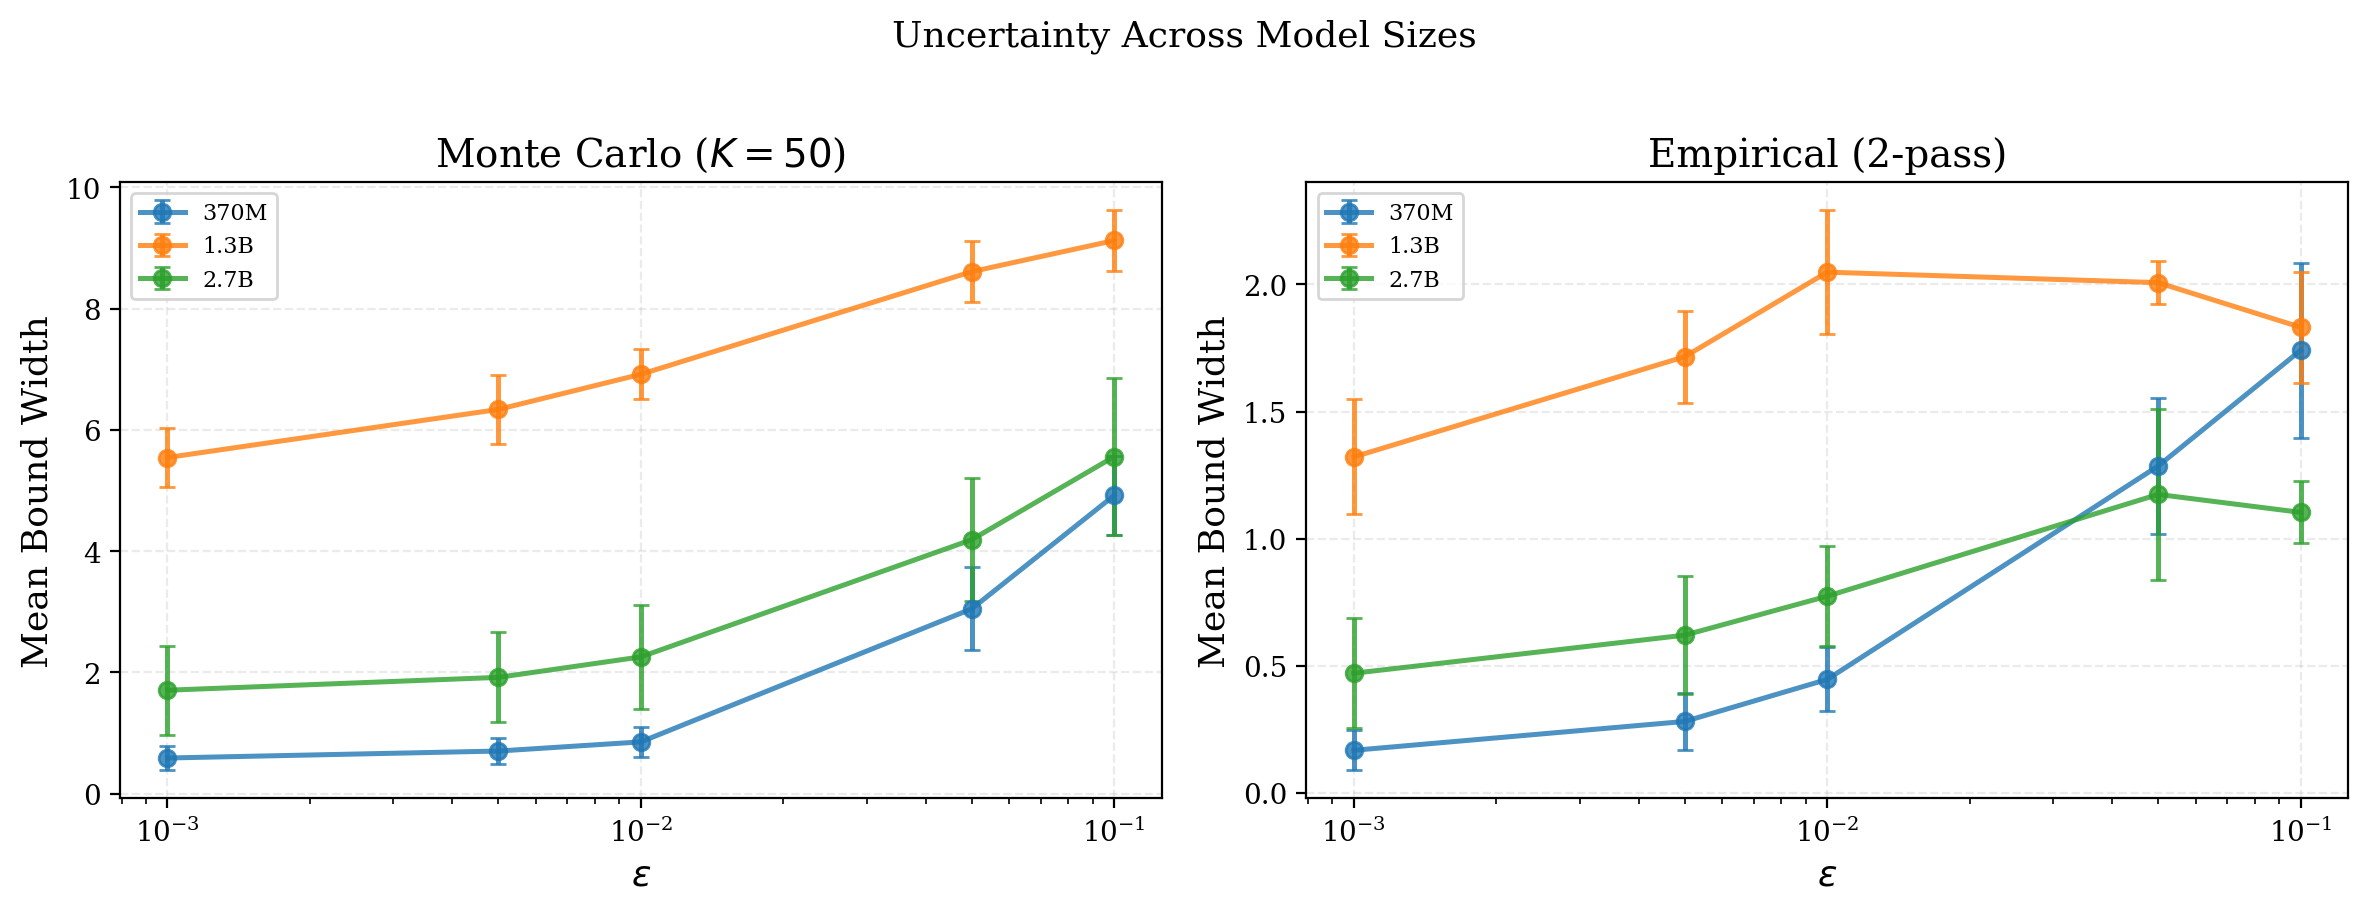
\includegraphics[width=0.85\textwidth]{results/full/plots/cross_model.png}
    \caption{Empirical bound width across model sizes. Monte Carlo bounds ($K{=}50$, left) are 2--6$\times$ wider than two-pass bounds (right), confirming that corner points underestimate true uncertainty.}
    \label{fig:bound_width}
\end{figure}

\begin{table}[H]
    \centering
    \caption{Uncertainty metrics at $\varepsilon{=}0.01$ (mean $\pm$ std across prompts).}
    \label{tab:results}
    \begin{tabular}{lccc}
        \toprule
        \textbf{Metric} & \textbf{370M} & \textbf{1.3B} & \textbf{2.7B} \\
        \midrule
        MC bound width & $0.85{\pm}0.27$ & $6.92{\pm}0.50$ & $2.25{\pm}0.91$ \\
        Emp.\ bound width & $0.45{\pm}0.14$ & $2.05{\pm}0.27$ & $0.77{\pm}0.22$ \\
        Top-1 agreement (MC) & $0.62{\pm}0.15$ & $0.37{\pm}0.08$ & $0.58{\pm}0.12$ \\
        \bottomrule
    \end{tabular}
\end{table}

Key findings:

\begin{enumerate}[nosep]
    \item \textbf{Monte Carlo bounds grow with $\varepsilon$}: from $\sim$0.5 (at $\varepsilon{=}0.001$) to $\sim$5--10 (at $\varepsilon{=}0.1$), with sub-linear scaling.
    \item \textbf{Two-pass bounds underestimate uncertainty} by 2--6$\times$, as the model is non-monotonic in embedding space.
    \item \textbf{Top-1 stability degrades}: at $\varepsilon{=}0.01$, 38--62\% of tokens retain the same argmax prediction across the perturbation set.
\end{enumerate}

\subsection{Model Size Does Not Monotonically Predict Robustness}

A surprising finding is the U-shaped relationship between model size and uncertainty: the 1.3B model exhibits \textbf{higher} bound widths (6.92 at $\varepsilon{=}0.01$) than both the smaller 370M variant (0.85) and the larger 2.7B variant (2.25). This suggests architectural factors beyond parameter count --- possibly related to the hidden dimension (2048 for 1.3B vs.\ 1024 for 370M and 2560 for 2.7B) and the corresponding Lipschitz constant of the weight matrices --- dominate perturbation sensitivity.

\subsection{Token-Level Uncertainty Patterns}

\begin{figure}[H]
    \centering
    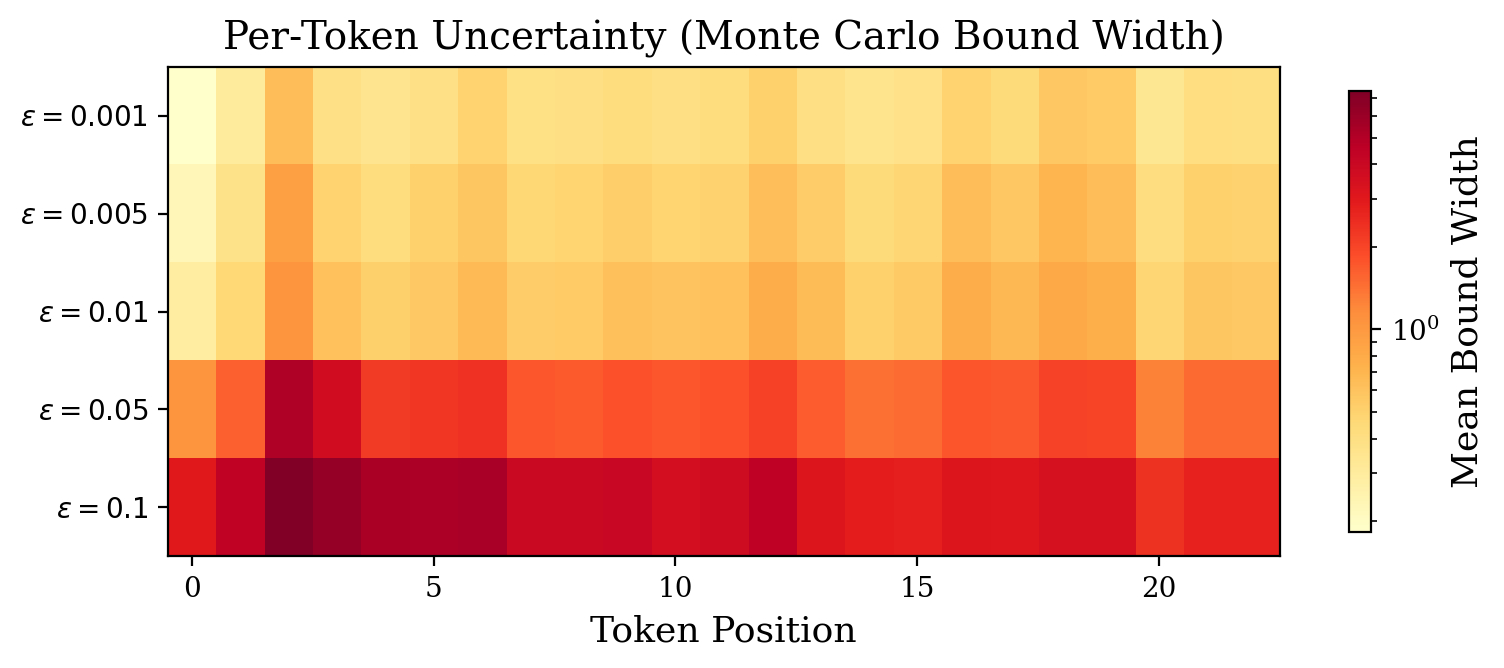
\includegraphics[width=0.75\textwidth]{results/full/plots/MMfreeLM-370M/token_uncertainty.png}
    \caption{Per-token MC bound width for MMfreeLM-370M. Later tokens exhibit higher uncertainty due to recurrent error accumulation. Some token positions show consistently higher sensitivity, possibly corresponding to semantically ambiguous tokens.}
    \label{fig:token}
\end{figure}

Figure~\ref{fig:token} shows per-token uncertainty across sequence positions. Later tokens generally show higher uncertainty, consistent with the compounding effect of recurrent state propagation through time. Some token positions consistently show elevated uncertainty, likely corresponding to semantically ambiguous or syntactically surprising tokens.

\section{Discussion}

\subsection{The Certification Gap}

Our results reveal a stark gap between certified and empirical UQ for recurrent LLMs. IBP bounds, while theoretically sound, explode within a single layer due to compounding conservatism in normalization and recurrence. This is not a bug but a fundamental limitation: RMSNorm's non-convex normalization surface and the multiplicative gating in the recurrence $o_t = f_t o_{t-1} + i_t$ amplify interval widths exponentially.

This ``certification gap'' mirrors the well-known challenge in adversarial robustness for image classifiers~\cite{zhang2020} but is amplified by recurrent architectures. Closing this gap for LLMs likely requires: (a) exploiting the scale-invariance of RMSNorm for tighter bounds, (b) CROWN-style linear relaxation for non-recurrent portions, or (c) input-level certification at the token rather than embedding level.

\subsection{Why Is the 1.3B Model More Sensitive?}

The 1.3B model exhibits 2--8$\times$ higher uncertainty than the 370M and 2.7B variants. A possible explanation lies in the model architecture: the 1.3B uses a hidden dimension of 2048 (vs.\ 1024 for 370M and 2560 for 2.7B). The weight matrix norms $\|\mathbf{W}\|_\infty$ scale approximately with $\sqrt{d_{\text{hidden}}}$, affecting the Lipschitz constant of each layer. Combined with different training dynamics (the 1.3B may have converged to a sharper minimum), this could explain the non-monotonic robustness pattern.

\subsection{Limitations}

Our study has several limitations: (1) we perturb embeddings rather than discrete tokens, which is well-defined mathematically but may not correspond to realistic input perturbations; (2) MC sampling with $K{=}50$ may miss rare extreme outputs; (3) we focus exclusively on MMfreeLM, which uses a specific recurrent architecture --- findings may differ for transformer-based or state-space models; (4) we do not perform IBP training~\cite{gowal2018}, which could produce models with tighter certifiable bounds.

\section{Conclusion}

We presented the first study of certified and empirical uncertainty quantification for matmul-free language models via bound propagation. Our key findings are:

\begin{enumerate}[nosep]
    \item \textbf{Certified IBP bounds explode} within 1 layer for recurrent LLMs due to RMSNorm and gated recurrence; this is a fundamental limitation requiring new techniques.
    \item \textbf{Monte Carlo empirical bounds} provide stable UQ: output logit widths of 0.5--10 under $\varepsilon \in [0.001, 0.1]$ perturbations.
    \item \textbf{Model size does not monotonically predict robustness}; the 1.3B model is 2--3$\times$ more sensitive than both the 370M and 2.7B variants.
    \item The \textbf{certification gap} in LLM verification is large, motivating tighter bound propagation for normalization and recurrent layers.
\end{enumerate}

Our implementation is open-source and extensible to other language model architectures.

\begin{thebibliography}{10}

\bibitem{hgrn2024}
Z.~Qin, S.~Yang, and Y.~Zhong.
\newblock HGRN2: Gated Linear RNNs with State Expansion.
\newblock \emph{arXiv:2404.07904}, 2024.

\bibitem{gowal2018}
S.~Gowal, K.~Dvijotham, R.~Stanforth, et al.
\newblock On the effectiveness of interval bound propagation for training verifiably robust models.
\newblock \emph{arXiv:1810.12715}, 2018.

\bibitem{zhang2020}
H.~Zhang, H.~Chen, C.~Xiao, et al.
\newblock Towards Stable and Efficient Training of Verifiably Robust Neural Networks.
\newblock In \emph{ICLR}, 2020.

\bibitem{zhang2018}
H.~Zhang, T.-W.~Weng, P.-Y.~Chen, C.-J.~Hsieh, and L.~Daniel.
\newblock Efficient Neural Network Robustness Certification with General Activation Functions.
\newblock In \emph{NeurIPS}, 2018.

\bibitem{zhu2023}
R.-J.~Zhu, Q.~Zhao, G.~Li, and J.~K.~Eshraghian.
\newblock SpikeGPT: Generative Pre-trained Language Model with Spiking Neural Networks.
\newblock \emph{arXiv:2302.13939}, 2023.

\end{thebibliography}

\end{document}
